\section{Wireframes}

\subsection{ Pantalla Principal de Selección de Rol}
\begin{samepage}\small
Esta es la primera pantalla que encuentra el usuario al abrir la aplicación, funcionando como un portal de bienvenida y un punto de navegación inicial. Su propósito es segmentar a los usuarios desde el principio, permitiendo que cada tipo de usuario acceda a su respectivo flujo de inicio de sesión de manera clara y directa. Este diseño evita una interfaz de login genérica y confusa, que requeriría que el usuario especifique su rol mediante un menú desplegable, simplificando así el primer paso de interacción con la aplicación.
\begin{figure}[H]
    \centering
    \IfFileExists{./Media/Wireframes/Page Main.png}{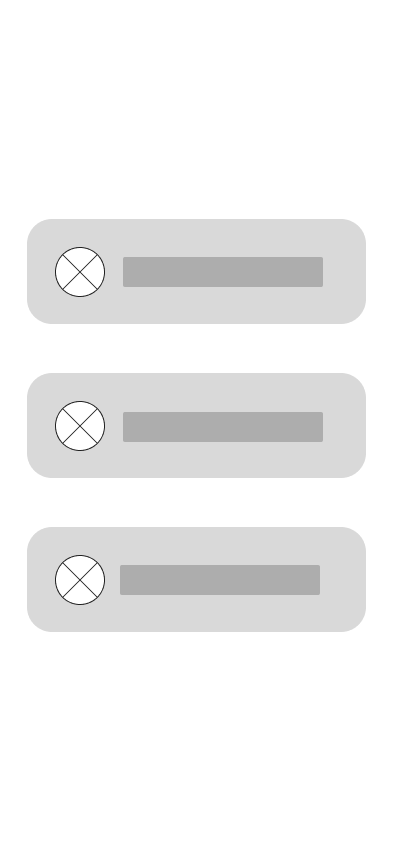
\includegraphics[width=0.28\textwidth]{./Media/Wireframes/Page Main.png}}{\fbox{\parbox{0.28\textwidth}{\centering Imagen ``Page Main.png'' no disponible}}}
    \caption{Wireframe de la pantalla de selección de rol.}\label{fig:wf-main}
\end{figure}
    \subsubsection*{Análisis de Componentes y Diseño}
    El diseño se basa en la simplicidad y la claridad. La pantalla presenta tres botones de selección de gran tamaño, dispuestos verticalmente, optimizados para una fácil interacción en dispositivos móviles donde el espacio táctil es primordial. Cada botón está diseñado para representar un rol principal (Estudiante, Docente y Padre de Familia) y reserva un espacio para un icono representativo que ayuda en la identificación visual rápida, junto con un área para el texto descriptivo del rol. La ausencia de otros elementos en la pantalla centra toda la atención del usuario en una única decisión: identificar su perfil.
    
    \subsubsection*{Flujo de Usuario y Funcionalidad}
    El flujo es directo y sin fricciones. El usuario identifica visualmente su rol, pulsa la opción correspondiente y la aplicación lo redirige a la pantalla de inicio de sesión específica para ese perfil. Este paso previo es crucial para personalizar la experiencia del usuario desde el primer momento. Al segmentar los flujos, la aplicación puede presentar a cada usuario únicamente la información y las herramientas que son relevantes para él, simplificando las interfaces subsecuentes y reduciendo la carga cognitiva.
\normalsize\end{samepage}
\clearpage

\subsection{ Pantalla de Inicio de Sesión (Estudiante)}
\begin{samepage}\small
Tras seleccionar el rol ``Estudiante'', el usuario es dirigido a esta interfaz de autenticación. Su diseño es limpio y centrado en la tarea, eliminando cualquier distracción para facilitar un acceso rápido y seguro a la plataforma. El uso del correo institucional como método de identificación estandariza el acceso para todo el alumnado, utilizando una credencial que ya les es familiar y que forma parte de su identidad digital dentro de la universidad.
\begin{figure}[H]\centering
    \IfFileExists{./Media/Wireframes/Login Student.png}{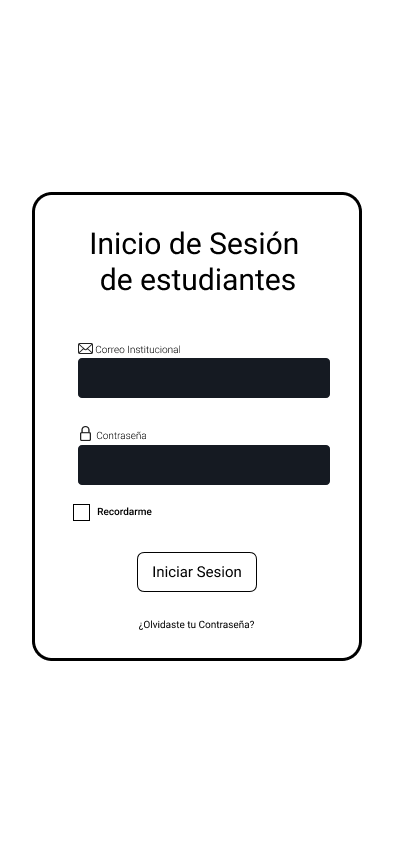
\includegraphics[width=0.28\textwidth]{./Media/Wireframes/Login Student.png}}{\fbox{\parbox{0.28\textwidth}{\centering Imagen ``Login Student.png'' no disponible}}}
    \caption{Wireframe de la pantalla de inicio de sesión para estudiantes.}\label{fig:wf-login-student}
\end{figure}
    \subsubsection*{Análisis de Componentes y Diseño}
    La jerarquía visual de la pantalla guía al usuario de forma natural. Incluye un título claro (``Inicio de Sesión de estudiantes''), seguido de dos campos de entrada bien definidos para ``Correo Institucional'' y ``Contraseña''. El checkbox para ``Recordarme'' es una función de conveniencia que reduce la fricción en usos futuros. El botón de acción principal (CTA) ``Iniciar Sesion'' está prominentemente ubicado, y un enlace discreto para recuperar la contraseña ofrece una solución a un problema común sin desviar la atención de la tarea principal.
    
    \subsubsection*{Flujo de Usuario y Funcionalidad}
    El usuario introduce sus credenciales para ser validado por el sistema. Esta pantalla actúa como una puerta de seguridad para proteger la información personal del alumno. Si la autenticación es correcta, el sistema le da acceso directo a su Panel del Alumno, su centro de información personal. En caso de error, se mostraría un mensaje informativo y no intrusivo para guiarlo en la corrección de los datos, evitando la frustración.
\normalsize\end{samepage}
\clearpage

\subsection{ Panel del Alumno}
\begin{samepage}\small
Esta pantalla es el centro de información principal para el estudiante; una herramienta de autogestión que le permite estar al tanto de su rendimiento y fomenta la responsabilidad sobre su asistencia. El diseño busca empoderar al estudiante, dándole acceso transparente, inmediato y comprensible a sus datos de asistencia, lo cual es un objetivo clave del proyecto Argos.
\begin{figure}[H]\centering
    \IfFileExists{./Media/Wireframes/Page Student.png}{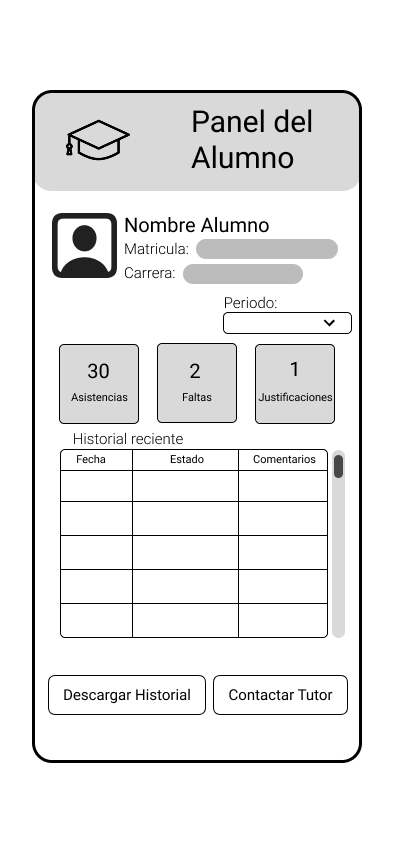
\includegraphics[width=0.28\textwidth]{./Media/Wireframes/Page Student.png}}{\fbox{\parbox{0.28\textwidth}{\centering Imagen ``Page Student.png'' no disponible}}}
    \caption{Wireframe del panel principal del alumno.}\label{fig:wf-student-panel}
\end{figure}
    \subsubsection*{Análisis de Componentes y Diseño}
    La interfaz presenta un encabezado con los datos del alumno (foto, nombre, matrícula), un selector para filtrar por periodo académico, tres tarjetas de resumen que ofrecen una vista cuantitativa inmediata de ``Asistencias'', ``Faltas'' y ``Justificaciones'', una tabla con el historial reciente para una revisión detallada, y botones de acción para ``Descargar Historial'' y ``Contactar Tutor''. El diseño prioriza la información más importante en la parte superior, permitiendo una lectura rápida y eficiente.
    
    \subsubsection*{Flujo de Usuario y Funcionalidad}
    Esta pantalla permite al estudiante verificar su estado de un solo vistazo, filtrar su historial por distintos periodos académicos, generar reportes oficiales en formato PDF para posibles trámites administrativos, e iniciar comunicación directa con su tutor para resolver dudas o aclarar inconsistencias. No es solo un repositorio de datos, sino una herramienta interactiva que promueve la autogestión.
\normalsize\end{samepage}
\clearpage

\subsection{ Pantalla de Inicio de Sesión (Docente)}
\begin{samepage}\small
Interfaz de autenticación diseñada específicamente para el personal docente de la institución. El uso de la matrícula como identificador asegura un método de acceso estandarizado y formal, alineado con los sistemas de gestión internos y diferenciando claramente el acceso del personal del de los alumnos. La consistencia visual con las otras pantallas de login reduce la curva de aprendizaje.
\begin{figure}[H]\centering
    \IfFileExists{./Media/Wireframes/Login Teacher.png}{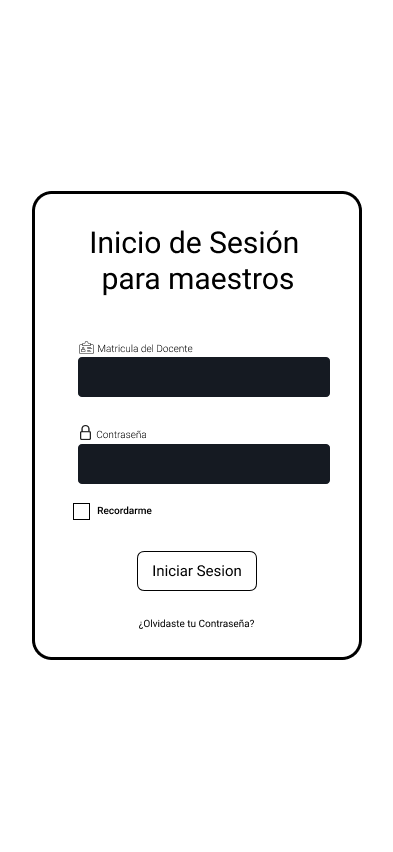
\includegraphics[width=0.28\textwidth]{./Media/Wireframes/Login Teacher.png}}{\fbox{\parbox{0.28\textwidth}{\centering Imagen ``Login Teacher.png'' no disponible}}}
    \caption{Wireframe de la pantalla de inicio de sesión para docentes.}\label{fig:wf-login-teacher}
\end{figure}
    \subsubsection*{Análisis de Componentes y Diseño}
    La pantalla contiene un título, un campo específico para la ``Matrícula del Docente'' como identificador único, un campo de contraseña y las opciones comunes que mantienen la consistencia en la experiencia de usuario a través de toda la aplicación (Recordarme, Iniciar sesión, ¿Olvidaste tu contraseña?). El diseño es deliberadamente simple para enfocarse en una única acción: la autenticación segura.
    
    \subsubsection*{Flujo de Usuario y Funcionalidad}
    El docente introduce su matrícula y contraseña para ser autenticado. Una vez validado, el sistema le concede acceso a sus herramientas de gestión de asistencia, como el panel de pase de lista. Este paso de validación es una medida de seguridad crítica para asegurar que la información sensible de los alumnos solo sea accesible y modificable por personal autorizado.
\normalsize\end{samepage}
\clearpage

\subsection{ Panel del Docente (Pase de Lista)}
\begin{samepage}\small
Esta es la herramienta principal y de uso diario para los maestros. Su diseño está optimizado para que el proceso de registrar la asistencia en el aula sea una tarea rápida, eficiente y con una mínima carga cognitiva, permitiendo al docente enfocarse en sus alumnos en lugar de en la herramienta administrativa. El objetivo es que el pase de lista tome solo un par de minutos al inicio de la clase.
\begin{figure}[H]\centering
    \IfFileExists{./Media/Wireframes/Page Teacher.png}{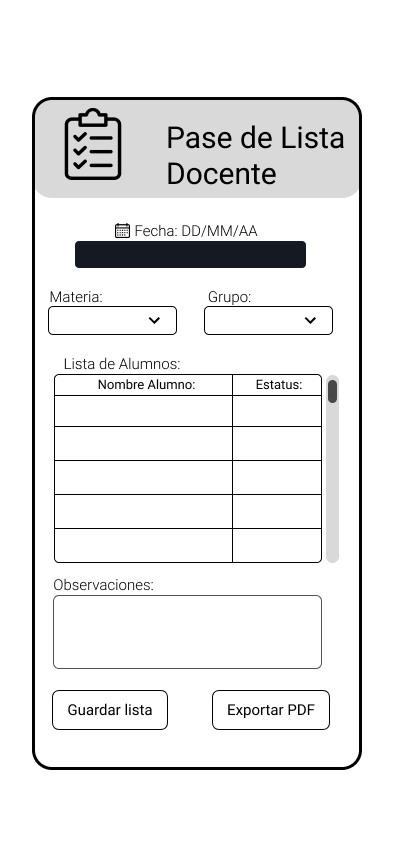
\includegraphics[width=0.28\textwidth]{./Media/Wireframes/Page Teacher.png}}{\fbox{\parbox{0.28\textwidth}{\centering Imagen ``Page Teacher.png'' no disponible}}}
    \caption{Wireframe del panel de pase de lista del docente.}\label{fig:wf-teacher-panel}
\end{figure}
    \subsubsection*{Análisis de Componentes y Diseño}
    La interfaz incluye selectores desplegables para ``Materia'' y ``Grupo'' que actúan como filtros para cargar la lista de alumnos correcta, un campo de ``Fecha'', la lista de alumnos con su estatus, un área de texto para ``Observaciones'' y los botones de acción ``Guardar lista'' y ``Exportar PDF''. La disposición vertical de los elementos guía al docente a través del proceso de forma lógica, de arriba hacia abajo.
    
    \subsubsection*{Flujo de Usuario y Funcionalidad}
    El flujo de trabajo es lineal e intuitivo: el docente selecciona la clase y grupo, la aplicación carga la lista de estudiantes correspondiente, el docente registra el estatus de cada alumno, añade notas generales si es necesario (ej. ``Actividad de laboratorio''), y finalmente guarda el registro del día en la base de datos o lo exporta para sus archivos personales.
\normalsize\end{samepage}
\clearpage

\subsection{ Pantalla de Inicio de Sesión (Padres de Familia)}
\begin{samepage}\small
Pantalla de acceso para los padres o tutores, diseñada para permitirles el monitoreo del estudiante de una forma segura y controlada. El uso de la matrícula del alumno como una referencia directa es una decisión de diseño clave para asegurar que el padre se vincule inequívocamente con la información de su hijo, garantizando la privacidad y la correcta asignación de datos.
\begin{figure}[H]\centering
    \IfFileExists{./Media/Wireframes/Login Parents.png}{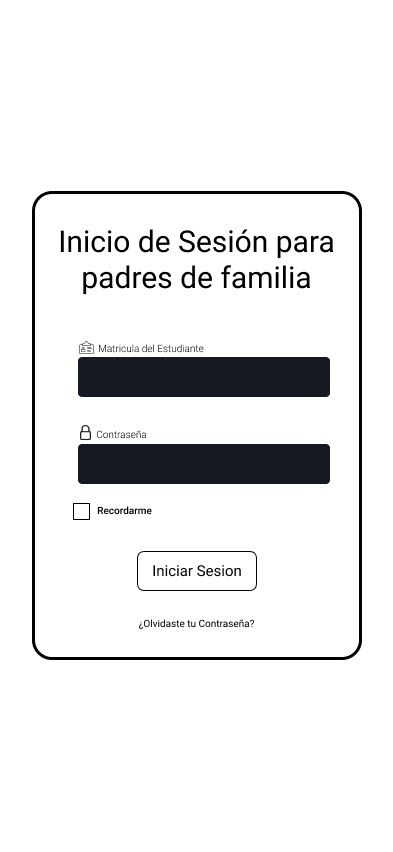
\includegraphics[width=0.28\textwidth]{./Media/Wireframes/Login Parents.png}}{\fbox{\parbox{0.28\textwidth}{\centering Imagen ``Login Parents.png'' no disponible}}}
    \caption{Wireframe de la pantalla de inicio de sesión para padres.}\label{fig:wf-login-parents}
\end{figure}
    \subsubsection*{Análisis de Componentes y Diseño}
    La interfaz incluye el título, un campo clave para la ``Matrícula del Estudiante'' que se va a consultar, el campo de contraseña y las opciones comunes de inicio de sesión. La simplicidad del diseño busca acomodar a usuarios con diferentes niveles de habilidad tecnológica, enfocándose únicamente en la información esencial para el acceso.
    
    \subsubsection*{Flujo de Usuario y Funcionalidad}
    El padre de familia se autentica utilizando la matrícula de su hijo o tutelado y su propia contraseña. Este método de doble factor (algo que el alumno tiene y algo que el padre sabe) asegura que solo tenga acceso a la información del estudiante correcto, respetando la privacidad de los datos, para después ingresar al panel de seguimiento.
\normalsize\end{samepage}
\clearpage

\subsection{ Panel de Padres de Familia}
\begin{samepage}\small
Interfaz diseñada para que los padres puedan consultar y visualizar de manera sencilla el historial de asistencia de sus hijos. Actúa como un puente de comunicación y seguimiento entre el hogar y la institución, fomentando una colaboración proactiva en la educación del alumno y aumentando la transparencia, uno de los objetivos del proyecto.
\begin{figure}[H]\centering
    \IfFileExists{./Media/Wireframes/Page Parents.png}{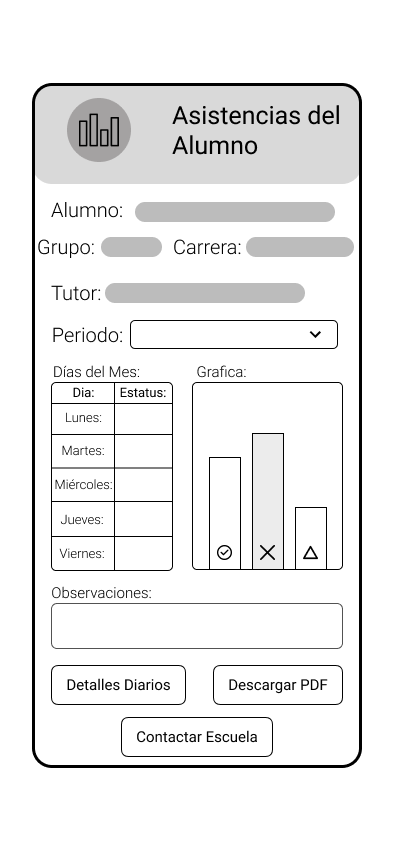
\includegraphics[width=0.28\textwidth]{./Media/Wireframes/Page Parents.png}}{\fbox{\parbox{0.28\textwidth}{\centering Imagen ``Page Parents.png'' no disponible}}}
    \caption{Wireframe del panel de seguimiento para padres.}\label{fig:wf-parents-panel}
\end{figure}
    \subsubsection*{Análisis de Componentes y Diseño}
    La pantalla muestra la información del alumno, una tabla de estatus por día para revisión detallada, y una gráfica de barras para un resumen visual rápido que facilita la identificación de patrones o tendencias (ej. ausencias recurrentes en un día específico). Los botones de acción ``Detalles Diarios'', ``Descargar PDF'' y ``Contactar Escuela'' están claramente visibles para promover la acción.
    
    \subsubsection*{Flujo de Usuario y Funcionalidad}
    Permite a los padres revisar el historial de asistencia, visualizar tendencias a través de gráficos para una fácil interpretación, descargar reportes y contactar a la institución directamente desde la aplicación. Este flujo completo, desde la visualización de datos hasta la comunicación, cierra el ciclo de monitoreo y acción.
\normalsize\end{samepage}

\clearpage
\subsection{ Pantalla de Carga}
\begin{samepage}\small
Pantalla intermedia que mejora la experiencia de usuario al proporcionar retroalimentación visual durante los tiempos de espera del sistema. Su función es gestionar la percepción del tiempo, reduciendo la incertidumbre y la sensación de lentitud de la aplicación mientras se procesan datos en segundo plano.
\begin{figure}[H]\centering
    \IfFileExists{./Media/Wireframes/Page Loader.png}{
\includegraphics[width=0.28\textwidth]{./Media/Wireframes/Page Loader.png}}{\fbox{\parbox{0.28\textwidth}{\centering Imagen ``Page Loader.png'' no disponible}}}
    \caption{Wireframe de la pantalla de carga.}\label{fig:wf-loader}
\end{figure}
    \subsubsection*{Análisis de Componentes y Diseño}
    El diseño es minimalista para no distraer. Consiste en un contenedor circular en la parte superior, ideal para mostrar el logo de Argos y reforzar la marca incluso en tiempos de espera, y un indicador de carga animado (spinner) en la parte inferior, un símbolo universal de que un proceso está en curso, lo que comunica claramente el estado del sistema al usuario.
    
    \subsubsection*{Flujo de Usuario y Funcionalidad}
    Esta pantalla aparece automáticamente en momentos clave, como después de iniciar sesión o al solicitar un reporte pesado, para informar al usuario que la aplicación está funcionando y procesando su solicitud. Este estado intermedio es crítico para prevenir la frustración y el posible abandono de la tarea por parte del usuario, haciendo que la aplicación se sienta más robusta y responsiva.
\normalsize\end{samepage}